\chapter{Robotvezérlés környezete}
\section{Robotirányítás}
Robotirányításhoz szükséges, hogy legyen egy mechanikai rendszer, ez a robot azon részrendszere, amely az akciót valósítja meg. Az akció során szükség lehet a robot mozgatására a környezetben,
ezt a helyváltoztató berendezés végzi. Motorok, különböző mechanikai tagok teszik lehetővé a helyváltoztatást. A szenzoros rendszer belső állapota maga a mechanikai rendszer állapota, míg a külső állapot a környezet állapotát jellemzi.
Sokféle külső környezeti állapot létezik. Ahhoz, hogy a különböző környezeti tényezőket, például hőmérséklet, fényerősség, mágnesesség, láthatóvá és érzékelhetővé tegyük a robotunk számára, fel kell szerelni a megfelelő szenzorokkal.
A dolgozat során egy Mantis Q drónt (\ref{fig:mantisq}. ábra) használunk robotként, a többit szimuláljuk.

\begin{figure}
	\centering
	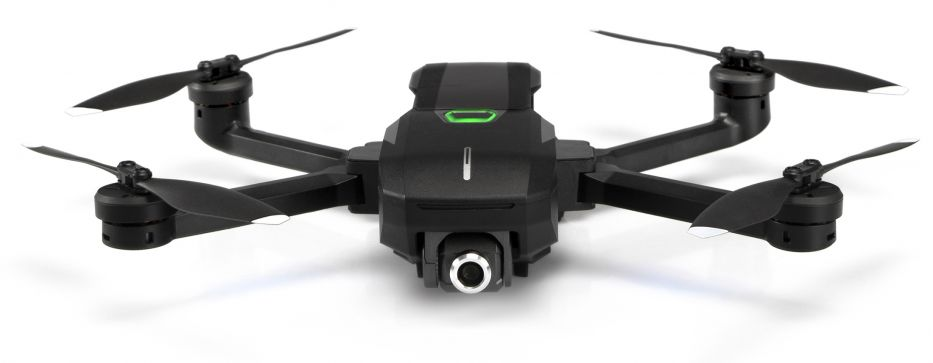
\includegraphics[width=\linewidth]{figures/mantisq.jpg}
	\caption{Yuneec Mantis Q \cite{mantisq}}
	\label{fig:mantisq}
\end{figure}

\section{Robot operációs rendszer - ROS}
Bármilyen robot rendelkezik különféle eszközökkel amivel érzékelik a világot és mozognak benne. A Robot operációs rendszer egy nyílt forráskódú könyvtárakat és eszközöket kínál a szoftverfejlesztés segítségére robotot, mint hardvert irányító alkalmazások létrehozásához. Hardver abszrakciót, driver-eket, könyvtárakat, megjelenítőket, üzenetek továbbítását, csomagkezelést és más szolgáltatást is nyújt. \cite{roswiki}
A ROS node-ok kommunikálni tudnak egymással, a szolgáltatások, hogy kérést küldjenek és választ kapjanak a node-ok között. A \emph{rosservice} szolgáltatással kapcsolódhatunk a ROS szerveréhez.
A \emph{roslaunch} utasítás egy .launch kiterjesztésű fájl alapján indít egy robotot, a megadott paraméterekkel.

\section{Kommunikáció - Mavros, Mavlink}
A MAVLink egy egyszerű üzenetküldési protokoll a drónokkal (és a fedélzeti drónkomponensek között) történő kommunikációhoz.A MAVLink hibrid publish-subscribe és point-to-point tervezési mintát követi. Az adatfolyamok témákként kerülnek elküldésre / közzétételre, míg a konfigurációs alprotokollok, például a missziók vagy a paraméterek point-to-point közötti újraküldéssel. Az üzeneteket az XML fájlok határozzák meg. Minden XML fájl meghatározza az adott MAVLink rendszer által támogatott üzenetkészletet. \cite{mavlink} A MAVLink nagyon hatékony, extrém kicsi az overhead, így QoS célra ideális. \\
\noindent
A mavros egy ROS kiegészítő, amely megvalósítja a MAVLink kommunikációját a ROS-t futtató számítógépek, a MAVLink-kompatibilis autopilotok és a MAVLink-kompatibilis Ground Control Station (GCS) között.

\section{Vezérlő - PX4}
A PX4 tág körben elterjedt mint robot vezérlő eszköz, akár egyéni, akár ipari felhasználásra. A nyílt forráskódú PX4 használható drón, de akár tengeralattjáró vagy hajó vezérlésére is, sőt könnyedén testreszabható eszközöket lehet vele készíteni, illetve megosztani a közösségi platformjukon. \cite{px4}
A ROS használható PX4-el és a Gazebo szimulátorral. A MAVROS MAVLink node-on keresztül használja a PX4-el való kommunikációhoz. A ROS és Gazebo integrált rendszer a \ref{fig:px4com} ábrán látható módon végzi a kommunikációt egy generikus PX4 szimulációs környezetben. A PX4 a szimulátorral (például Gazebo-val) kommunikál, ahonnan megkapja a szenzor adatot, esetünkben a kamera adatát a szimulált világból, illetve elküldi a motor és rotor vezérlési paramétereit. A PX4-el közvetlen fizikai eszközöket mozgatunk, ebben a környezetben a fejlesztő feladata, hogy megvalósítsa, hogy például egy méteres magasságba felszálláshoz a drónnak milyen eszközeivel mit kell csinálni. A PX4 továbbá kommunikál a GCS-el és a fedélzeti API-val, ami esetünkben a ROS, ahova parancsokat tud küldeni. \cite{px4dev}

\begin{figure}
	\centering
	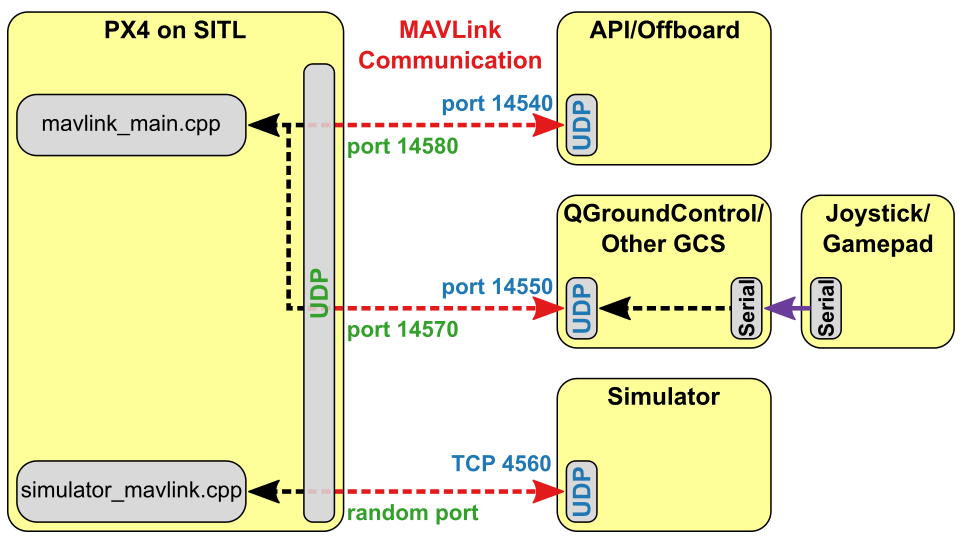
\includegraphics[width=\linewidth]{figures/px4_sitl_overview.png}
	\caption{PX4 kommunikációja Mavlink protokollal \cite{px4dev}}
	\label{fig:px4com}
\end{figure}

\section{Szimulációs környezet - Gazebo}
\begin{figure}
	\centering
	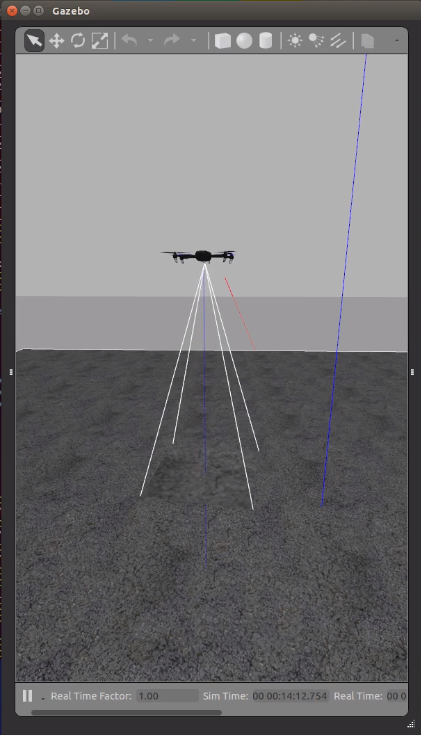
\includegraphics[height=12cm]{figures/sitl_optical_flow.png}
	\caption{Gazebo kamerás drón modell}
	\label{fig:sitl_optical_flow}
\end{figure}
Mivel a dolgozat egy nagy számú eszközkiszolgálást szeretne bemutatni és a tanszéknek egy Mantis Q drónja van, ezért a többinek a kiszolgálását szimulálni fogjuk, erre pedig kell egy szimulációs környezet, ami a Gazebo lesz. A Gazebo szimulátor lehetővé teszi az algoritmusok gyors tesztelését, a robotok tervezését, a regressziós tesztek elvégzését és akár AI rendszer kialakítását. Továbbá lehetőséget nyújt a robotok pontos és hatékony szimulálására komplex beltéri és kültéri környezetben. Kézhez kapunk egy 3D-s felületet is, amivel figyelni tudjuk a szimulációt, továbbá felhő alapú támogatást is biztosít, ami a témában még jól fog jönni.
A Gazebo különböző modelleket támogat, mint például a SITL optical flow, ami pont egy Mantis Q jellegű kamerás drónt szimulál bejövő és feldolgozható optikai adatcsomaggal (\ref{fig:sitl_optical_flow}. ábra). Az ábrán látható drónból kijövő fénykúp által vetődő keret lesz a kamera képe.
Sőt egy szimulált világba akármennyi modellt képesek vagyunk szimulálni a következőképpen.
\begin{lstlisting}[caption={10 optikai adatfolyamos drón szimulálása Gazebo-val}, label={lst:multi}]
cd src/Firmware
DONT_RUN=1 make px4_sitl_default gazebo
Tools/gazebo_multi_vehicle.sh -m sitl_optical_flow -n 10
\end{lstlisting}
\noindent
Az \ref{lst:multi}. számú listázásban futtatott script egyépként a szimulációs fájlrendszerben \emph{xacro} fájlokat módosítva éri el, hogy létrejöjjenek a kívánt modellek. Ezen a scripten könnyen lehet módosítani saját tetszésünk szerint. A modellek elérésének az UDP portjai 14560-tól, a TCP portjai 4560-tól inkrementálódnak, továbbá az összes a 14550 porton broadcast-el. \cite{multi-vehicle}

\noindent
A Gazebo felbontható szerverre és kliensre és a következő számításokat végzik:
\paragraph{Szerver}
\begin{itemize}
	\item Fizika kiszámítása
	\item Szenzorok szimulálása
	\item Engine API
\end{itemize}
\paragraph{Kliens}
\begin{itemize}
	\item Renderelés
	\item GUI
\end{itemize}

\section{Együttes működés}
A következő roslaunch utasítás egy lokális szimulációt indít a ROS-t összekötve MAVROS-al a \ref{fig:px4com}. ábrán látható módon keresztül.
\begin{lstlisting}[caption={Lokális PX4 szimuláció ROS-on keresztül Mavlink-el összekötve}]
roslaunch mavros px4.launch fcu_url:="udp://:14540@127.0.0.1:14557"
\end{lstlisting}
A szimulált világban való videót a QGroundControl alkalmazással lehet megfigyelni, továbbá akármennyi modell manuális irányítását is ezzel az eszközzel teszteltem. Persze a későbbi tömeges szimulációhoz, majd valamilyen automatizmusra lesz szükség. Az együttes működéshez szükséges egyfajta proxy, a mavlinken keresztül való kommunikációhoz, ami a Mavros (\ref{fig:egyuttes}. ábra).

\begin{figure}
	\centering
	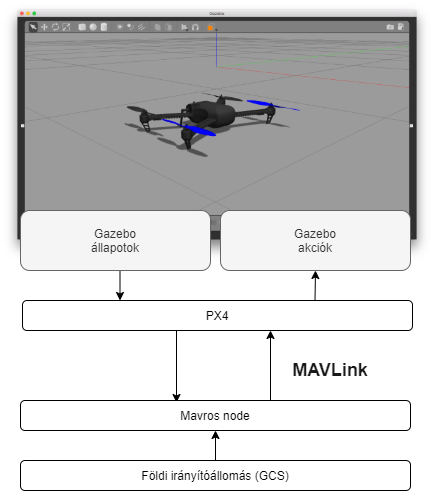
\includegraphics[height=10cm]{figures/egyuttes.png}
	\caption{Az együttes működés kommunikációja Mavros node-on keresztül}
	\label{fig:egyuttes}
\end{figure}